\documentclass[12pt, a4paper]{article}

\usepackage[T1]{fontenc}
\usepackage[left=3cm, right=3cm, top=4cm, bottom=4cm]{geometry}
\usepackage{setspace}
\usepackage{hyperref}
\usepackage{graphicx}
\graphicspath{./}

\renewcommand{\labelitemi}{-}

\newenvironment{itemlist}
{
  \vspace{-0.5\topsep}
  \begin{itemize}
    \setlength{\itemsep}{4pt}
    % \setlength{\topsep}{0pt}
    \setlength{\parskip}{0pt}
    % \setlength{\partopsep}{0pt}
} {
  \end{itemize}
  \vspace{-0.5\topsep}
}

\newcommand\code[1]{\texttt{#1}}

\title{Technical Documentation of Nebula \\
\large A comprehensive reference
}
\author{Piotr Kocia}
\date{}

\begin{document}
\maketitle

\tableofcontents

\section{Introduction}
Nebula is a realtime interactive user-driven desktop program for construction
and simulation of logic circuits. The program is not suitable for CAD
applications. Its intended use is for educational purposes.

\section{Requirements}
System requirements for Nebula:
\begin{itemlist}
  \item 64-bit Linux or Windows operating system,
  \item X Window System (X11) or Desktop Window Manager (DWM),
  \item OpenGL 4.5 core (GL) capable GPU and a compatible graphics driver.
\end{itemlist}
In order to properly utilise the program, external input devices are necessary,
namely a mouse and a keyboard. Nebula does not support other means of user
input.

\section{Overview}

\subsection{User Interface}
\begin{figure}
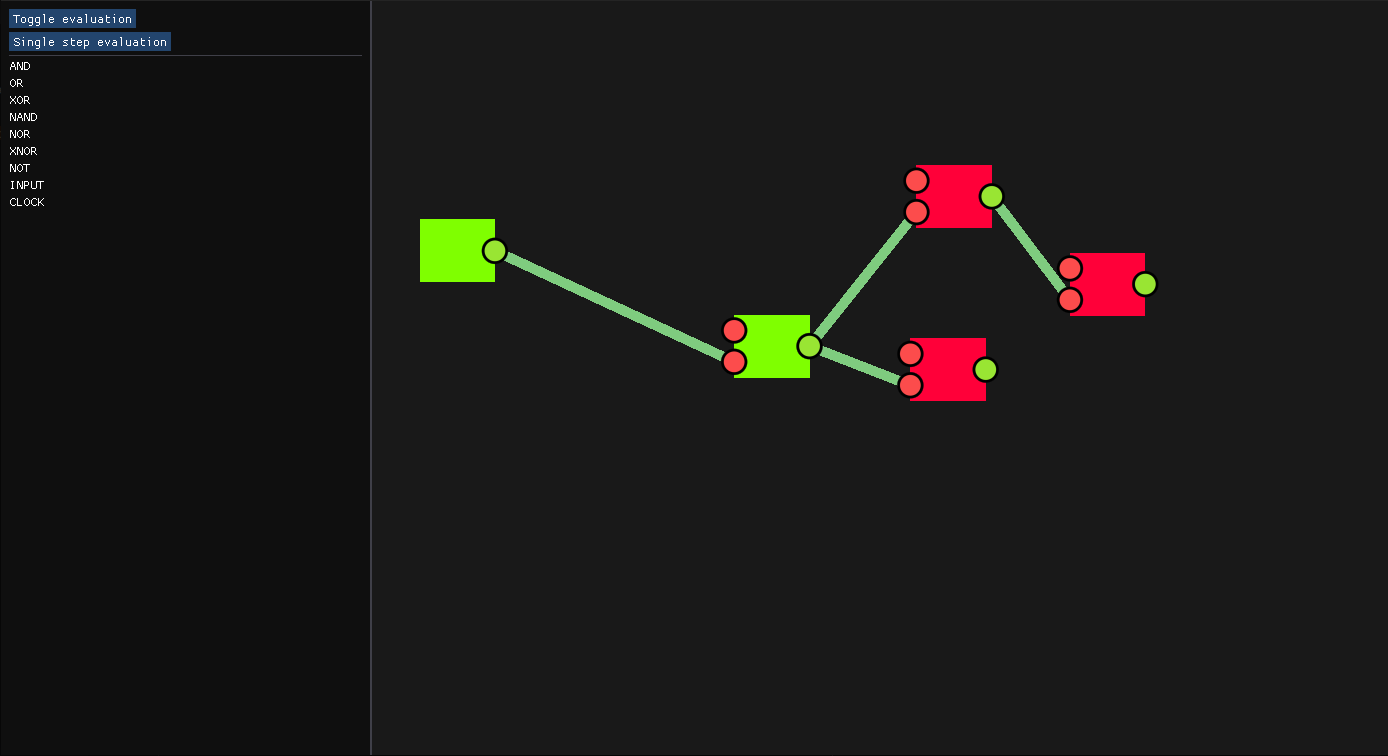
\includegraphics[width=\linewidth]{user_interface.png}
\caption{The user interface of Nebula.}
\end{figure}

The user inferface consists of two sections - viewport and toolbar.

\subsubsection{Toolbar}
The toolbar contains interactive buttons that allow the user to create new gates
or run the simulation. There is an option to run the evaluation continously or
run a single iteration of evaluation. The available gates are: AND, OR, XOR,
NAND, NOR, XNOR, NOT, INPUT, CLOCK.

\subsubsection{Viewport}
The viewport is the view into the scene presenting the layout of the logic
circuit. A user may move logic components around the scene, connect or
disconnect them, and delete or create new elements.

\begin{figure}
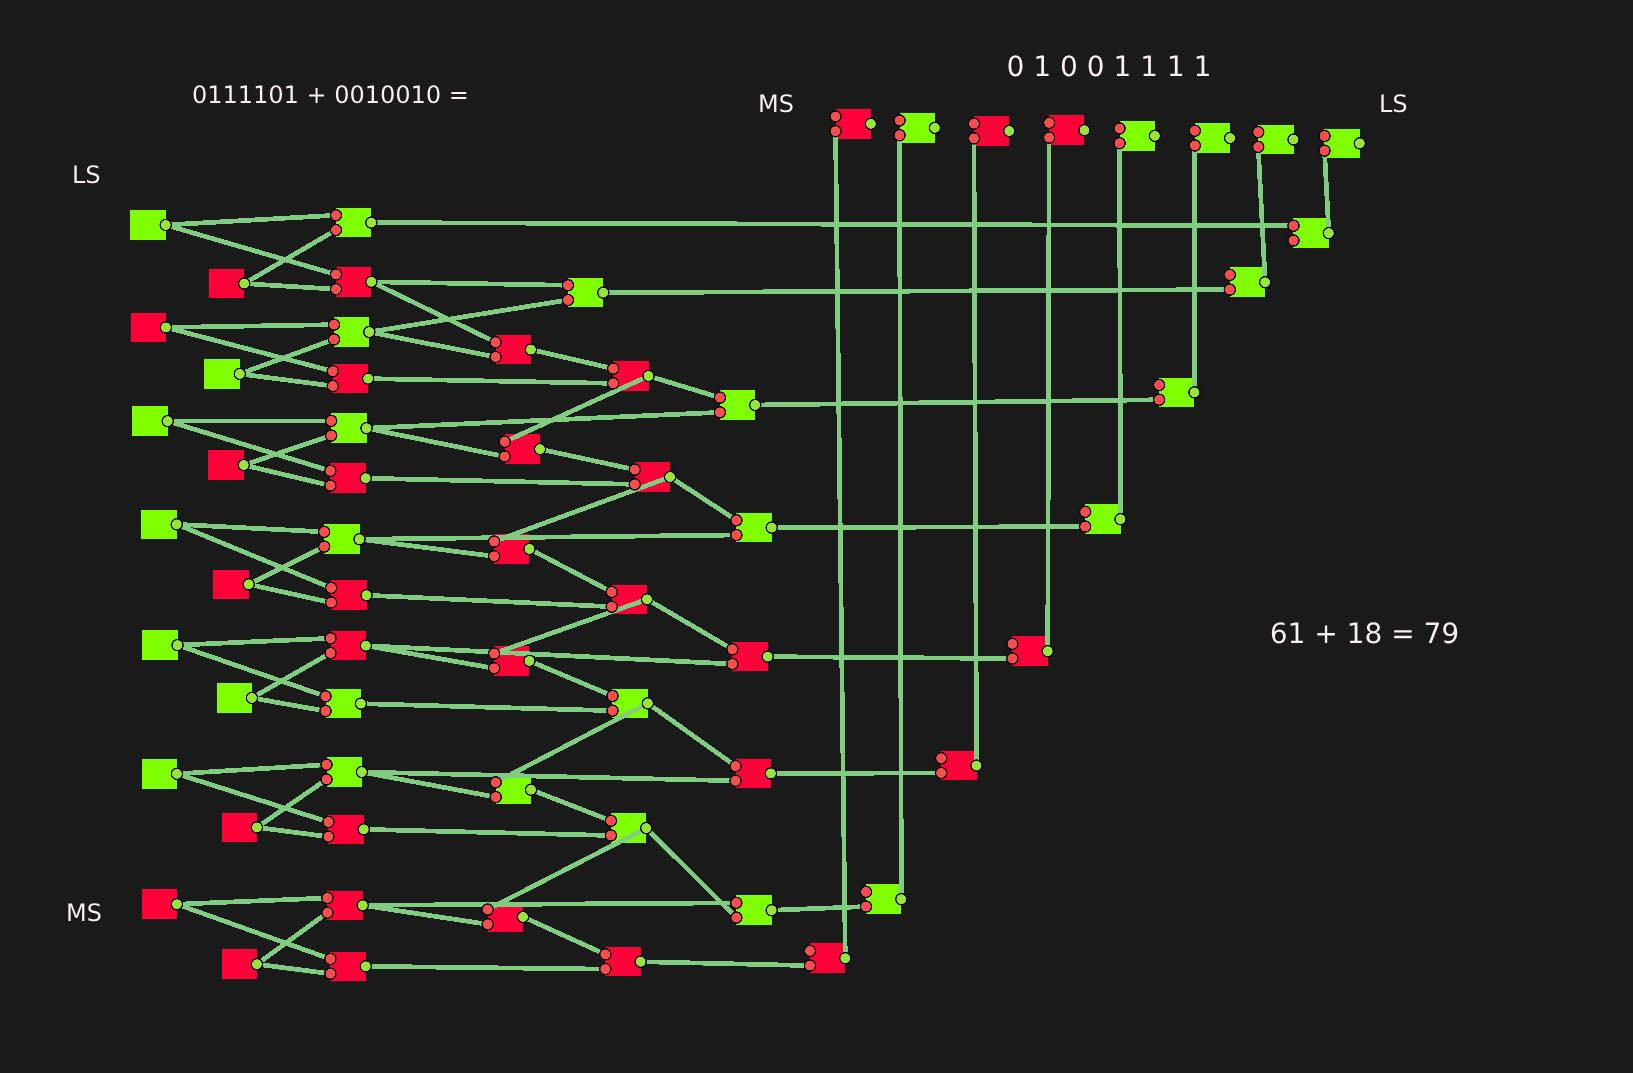
\includegraphics[width=\linewidth]{gate_example.jpg}
\caption{An example circuit with annotations.}
\end{figure}

\subsection{Simulation}
The real world is continuous and thus difficult to simulate, hence we use
simplifications and approximations that are widely acknowledged:
\begin{itemlist}
  \item Time is discretised. The smallest unit is 1 tick.
  \item All gates process their input simultaneously and take 1 tick to output
  new information.
  \item There are no transient states, all gates always have a valid state at
  every tick.
\end{itemlist}
Furthermore, the following uphold:
\begin{itemlist}
  \item A unconnected input is equivalent to always being \code{false}.
\end{itemlist}

\section{Glossary}
\subsection{General}
\begin{description}
  \item[Connection]
  Connection between two ports enabling transmission of boolean signals.
  \item[Evaluation]
  A single iteration of the computation of the new next state of a logic
  circuit in the current scene.
  \item[Gate]
  A unit of logic execution consuming boolean input and producing boolean
  output.
  \item[Port]
  An IO component of a gate allowing information to flow in or out. A port may be
  an in port or out port.
  \item[Scene]
  A collection of logic circuit elements.
  \item[Toolbox]
  A section of the user interface with user interface elements allowing
  interaction, such as adding gates or single-stepping evaluation.
  \item[Viewport]
  A user interface section displaying the scene.
  \item[World Space]
  An infinite virtual coordinate system where the elements of a logic circuit
  are placed.
\end{description}
\subsection{Gates}
\begin{description}
  \item[AND]
    Gate satisfying the AND boolean function.
    $$
    \begin{array}{|cc|c|}
    \hline
    A & B & Q \\
    \hline
    0 & 0 & 0 \\
    0 & 1 & 0 \\
    1 & 0 & 0 \\
    1 & 1 & 1 \\
    \hline
    \end{array}
    $$
  \item[OR]
    Gate satisfying the OR boolean function.
    $$
    \begin{array}{|cc|c|}
    \hline
    A & B & Q \\
    \hline
    0 & 0 & 0 \\
    0 & 1 & 1 \\
    1 & 0 & 1 \\
    1 & 1 & 1 \\
    \hline
    \end{array}
    $$
  \item[XOR]
    Gate satisfying the XOR boolean function.
    $$
    \begin{array}{|cc|c|}
    \hline
    A & B & Q \\
    \hline
    0 & 0 & 0 \\
    0 & 1 & 1 \\
    1 & 0 & 1 \\
    1 & 1 & 0 \\
    \hline
    \end{array}
    $$
  \item[NAND]
    Gate satisfying the NAND boolean function.
    $$
    \begin{array}{|cc|c|}
    \hline
    A & B & Q \\
    \hline
    0 & 0 & 1 \\
    0 & 1 & 1 \\
    1 & 0 & 1 \\
    1 & 1 & 0 \\
    \hline
    \end{array}
    $$
  \item[NOR]
    Gate satisfying the NOR boolean function.
    $$
    \begin{array}{|cc|c|}
    \hline
    A & B & Q \\
    \hline
    0 & 0 & 1 \\
    0 & 1 & 0 \\
    1 & 0 & 0 \\
    1 & 1 & 0 \\
    \hline
    \end{array}
    $$
  \item[XNOR]
    Gate satisfying the XNOR boolean function.
    $$
    \begin{array}{|cc|c|}
    \hline
    A & B & Q \\
    \hline
    0 & 0 & 1 \\
    0 & 1 & 0 \\
    1 & 0 & 0 \\
    1 & 1 & 1 \\
    \hline
    \end{array}
    $$
  \item[NOT]
    Gate satisfying the NOT boolean function.
    $$
    \begin{array}{|c|c|}
    \hline
    A & Q \\
    \hline
    0 & 1 \\
    1 & 0 \\
    \hline
    \end{array}
    $$
  \item[INPUT]
    Emits constant value. Toggleable.
  \item[CLOCK]
    Gate changing value every evaluation.
\end{description}

\end{document}
